\documentclass{amsart}
\usepackage{graphicx}
\graphicspath{{./}}
\usepackage{hyperref}
\usepackage{csvsimple}
\usepackage{longtable}
\usepackage{lscape}
\usepackage{epigraph}
\title{Zulf Goes Against Friedrich Nietzsche and Talcott Parsons} 
\author{Zulfikar Moinuddin Ahmed}
\date{\today}
\begin{document}
\maketitle

\section{Moral Values are Not Absorbed From Society}

Friedrich Nietzsche was obsessed about the idea that people's moral norms were absorbed from some leaders from some age, and he spoke of 'herd mentality' and 'slave morality' seeking some new values that are autonomously generated.  Talcott Parsons the sociologist spoke a half a century ago, according to Christopher Boehm, about 'internalisation' of group values.  

My recent results from World Values Survey are not consistent with these theories at all.  Moral Value distribution across the world, across ethnic, language, religion, and other barriers are remarkably uniform.  And this implies that internalisation of either group values or the following of a religious leader as a herd animal are both not parsimonious explanation of the remarkably uniform distributions of moral convictions across the world.  Rather, genetic evolution and holding and moral values as part of our evolutionary genetic heritage over millions of years have more sensible explanatory power.  

\section{Data}

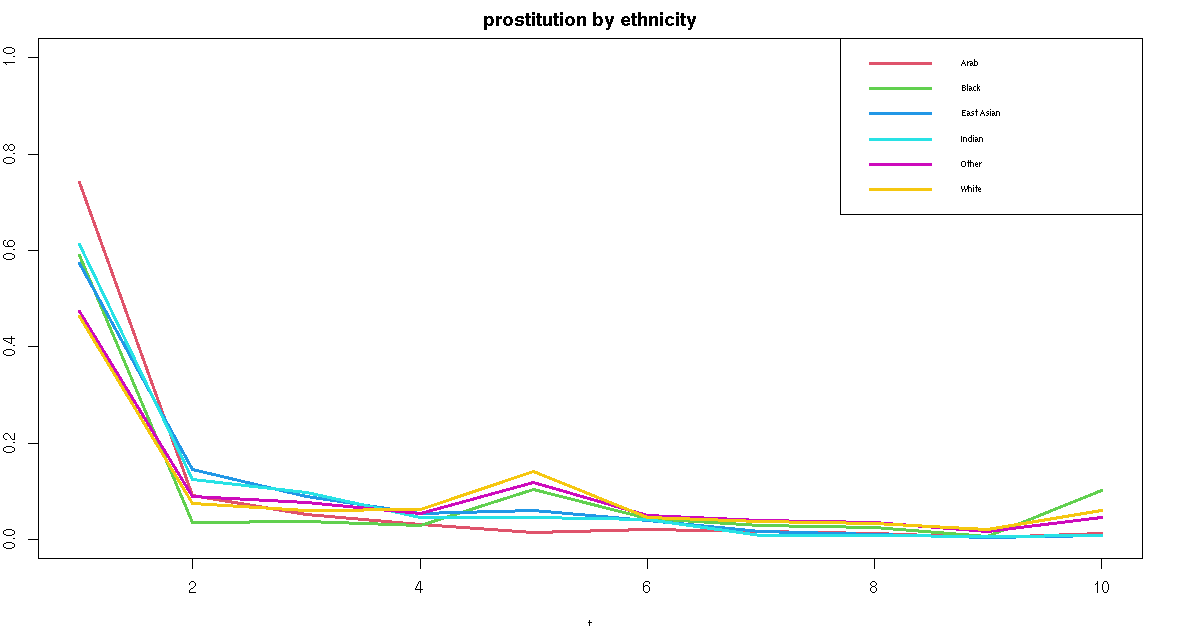
\includegraphics[scale=0.4]{nietzsche_parsons_prost.png}

\section{Conclusions}
The distribution of the particular convictions regarding prostitutions by ethnicity show a remarkable uniformity, and these are global.  No particular leader, no particular religion, no particular type of specific social values can explain this if they were purely externally generated and then absorbed.  The idea that we are malleable morally has been popular throughout the nineteenth and twentieth centuries.  At least for some moral questions like views about prostitution, there is a remarkable universality and it is too costly to produce this my external methods such as indoctrination or by producing propaganda for absorption by many people.  These sorts of ideas are interesting, I will admit, but the data above will not support these theories, and so I consider these sorts of theories successfully challenged.  The details of Friedrich Nietzsche and Talcott Parson's work are not necessary for this refutation of their main theses.

\end{document}